\newpage
\section{Notes on Section 4}

\subsubsection{Explaining Lemma 4.1}

A proof of Lemma 4.1 can also be found in the appendix of the original paper. However,
the relation between the norms is missing in the original paper - that is why we state it here again.
From 3.5 in the paper, we had:
\begin{align}
	\frac{1}{(L+1)^2} \pqnorm{\theta}{fr}{2} = \E{v^\TT X X^\TT v} = \E{\norm{f_\theta}^2}.
\end{align}
Remember that the output of the network, $f_\theta(x)$, is a vector in $\setreal^k$ of probabilities for each of the $k$ classes.  
For the Frobenius Norm of a Matrix $A$ and a vector $x$ the following holds.
\begin{align}
	\frobnorm{A} &\geq \spectralnorm{A} \\
	\frobnorm{x} &= \lnorm{x} = \spectralnorm{x} \\
	\spectralnorm{Ax} &\leq \spectralnorm{A} \cdot \lnorm{x} \\
\end{align}
It follows.
\begin{align}
	\E{\spectralnorm{f_\theta}^2}
	&= 
		\E{ \spectralnorm{f_\theta}^2} \\
	&= 
		\E{ \spectralnorm{\structuredNN}^{2} } \\
	&\leq 
		\E{ \spectralnorm{x}^2 \prod \spectralnorm{D^i(x)}^2 \prod \spectralnorm{W^i}^2 }.
\end{align}
Since $W^i$ is independent of the data $x$, it does not have to be inside the expectation.
\begin{align}
\frac{1}{(L+1)^2} \frnorm{\theta}^2
	&=
		\E{\spectralnorm{f_\theta}^2}  \\	
	&\leq 
		\E{ \spectralnorm{x}^2 \prod \spectralnorm{D^i(x)}^2 \prod \spectralnorm{W^i}^2 } \\
	&=
		\E{ \lnorm{x}^2 \prod_{t=1}^{L+1} \spectralnorm{D^t(x)}^2 } \prod_{t=0}^{L} \spectralnorm{W^i}^2
\end{align}
Now taking the root on both sides reveals Lemma 4.1 and concludes the explainiation.





\begin{figure}[htb]
	\centering
	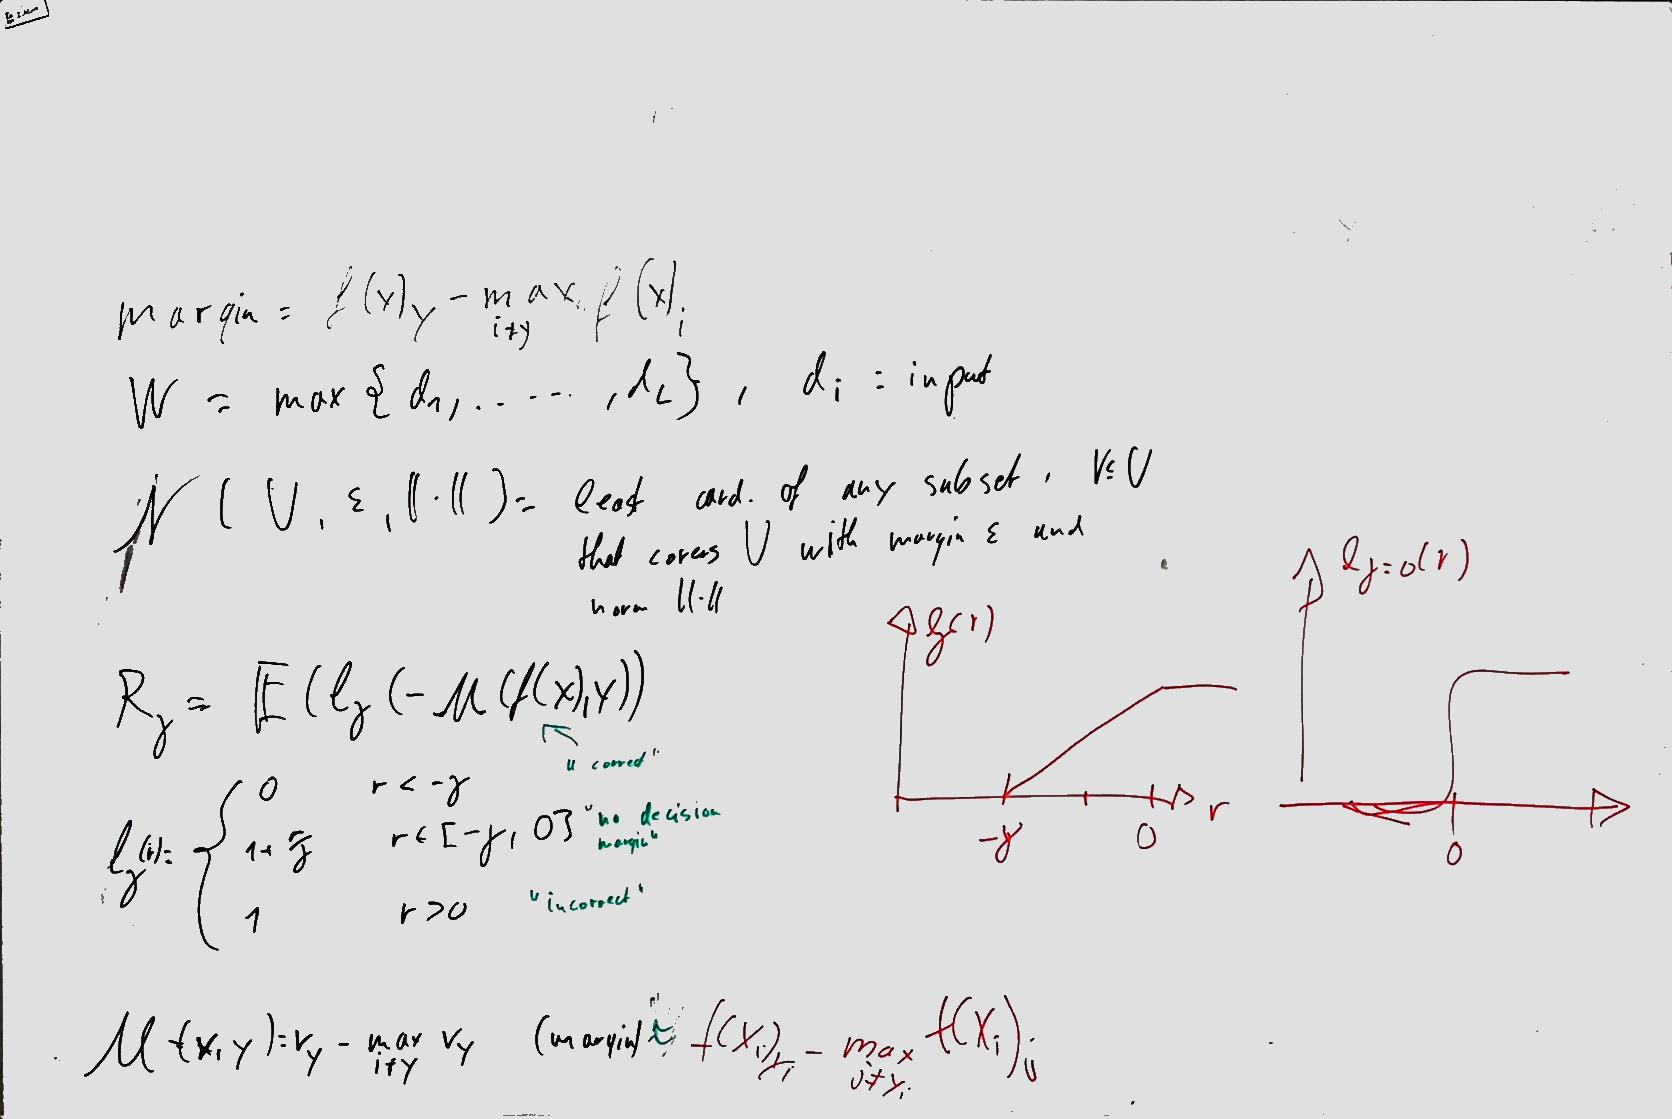
\includegraphics[width=\textwidth]{whiteboard_notes/18.jpg}
\end{figure}

\begin{figure}[htb]
	\centering
	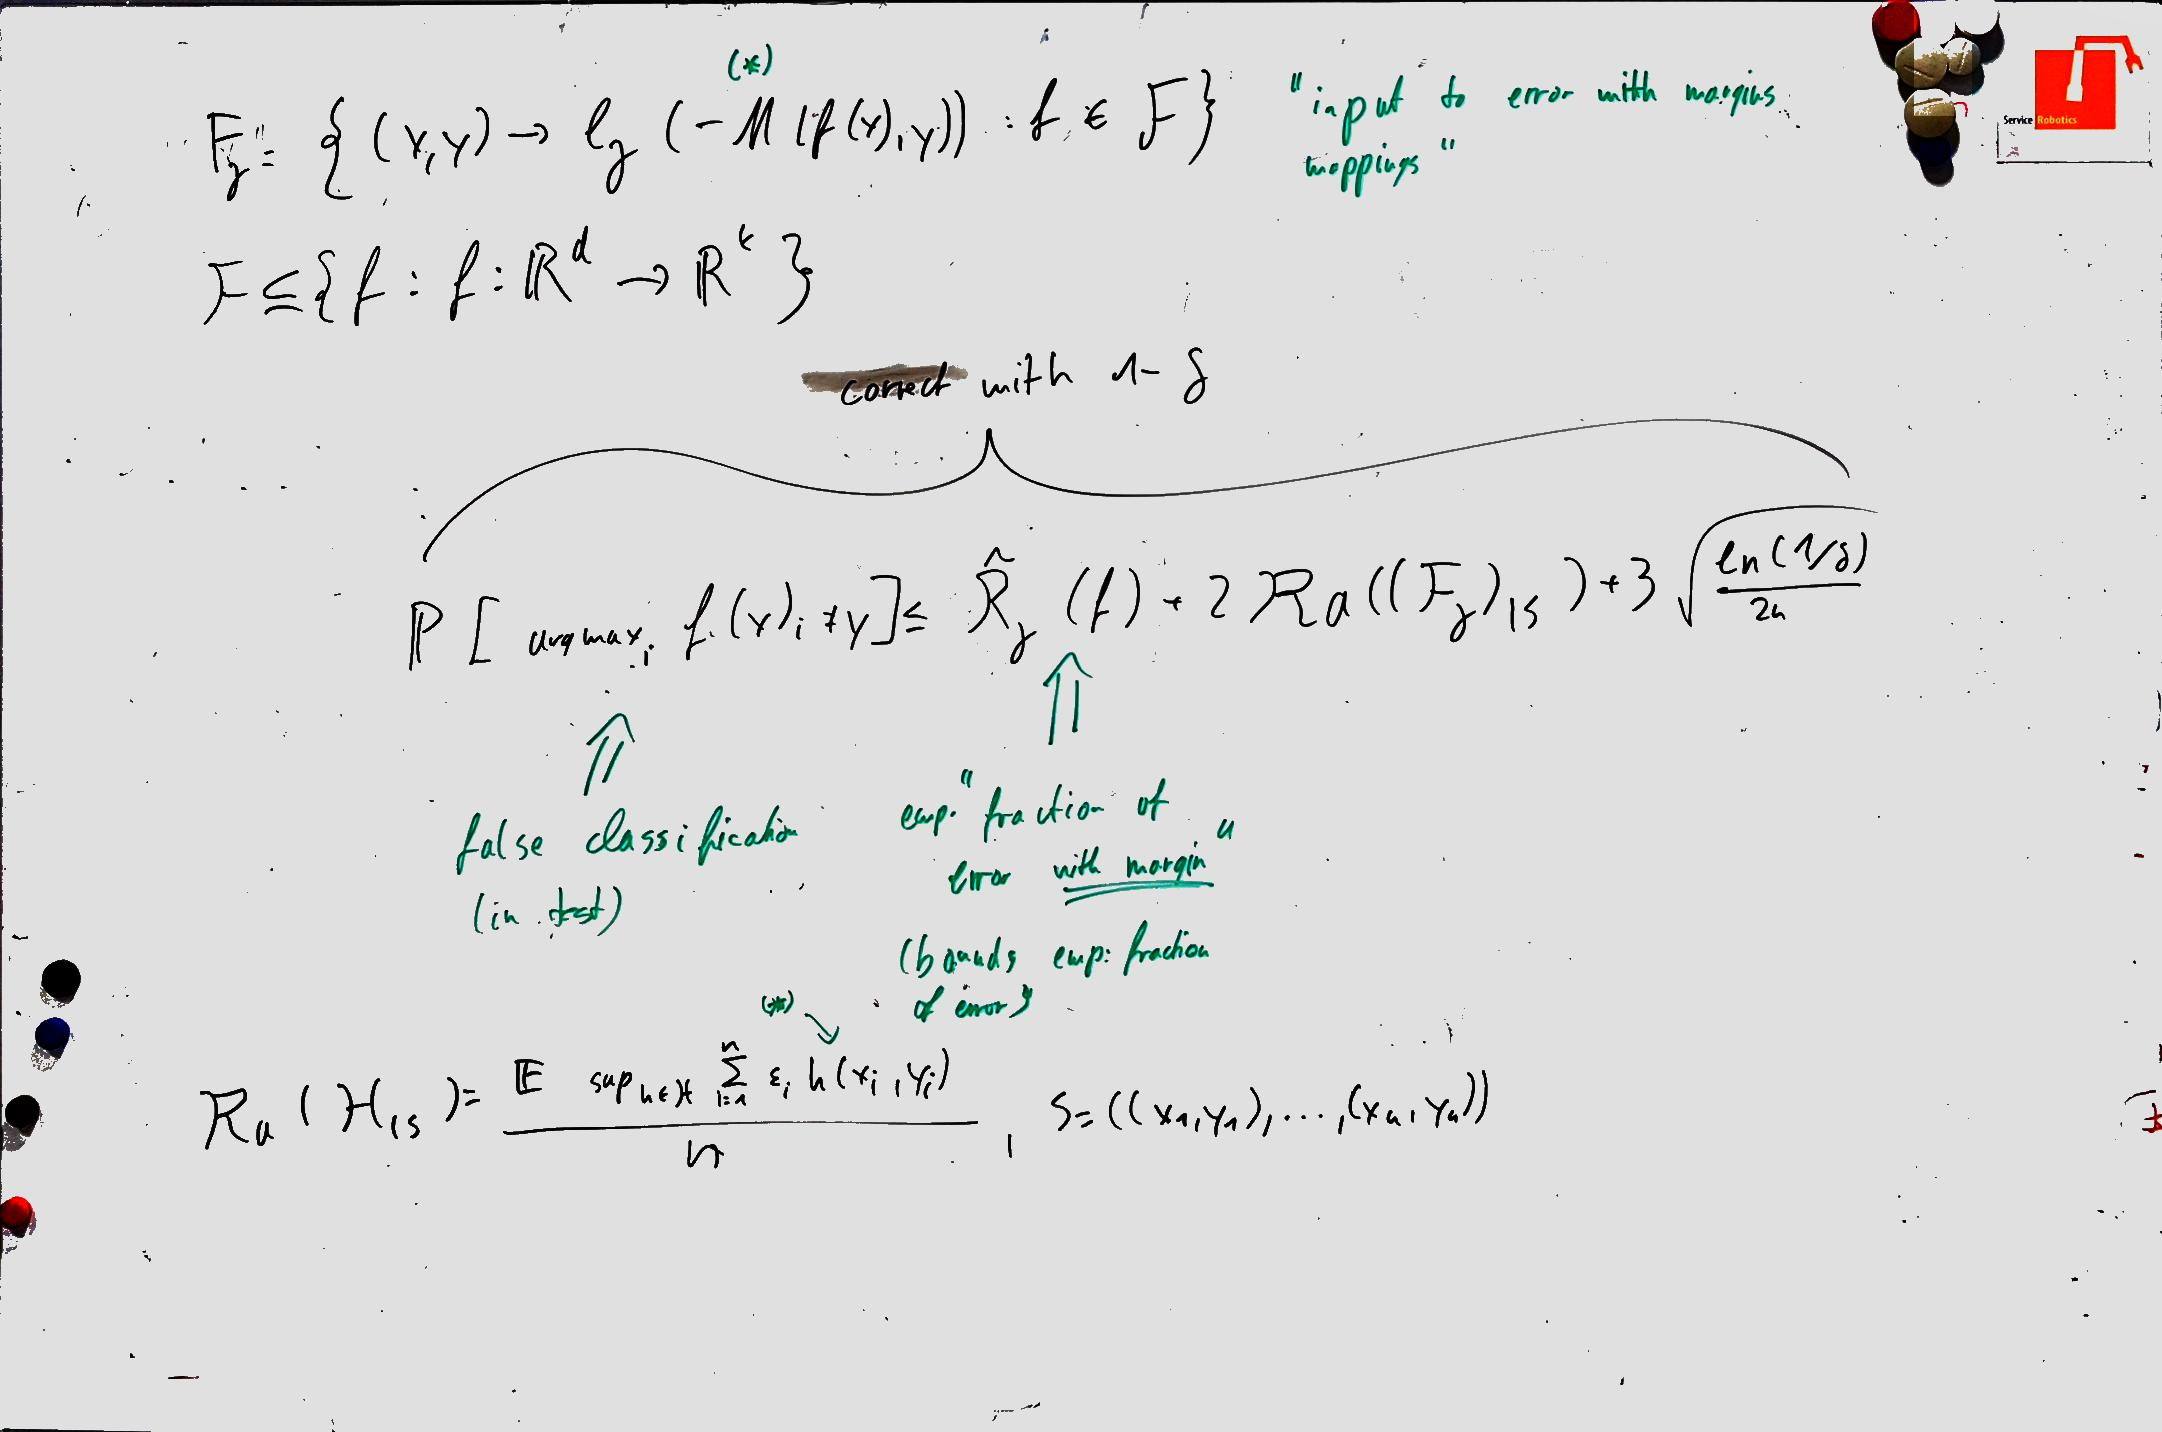
\includegraphics[width=\textwidth]{whiteboard_notes/19.jpg}
\end{figure}

\begin{figure}[htb]
	\centering
	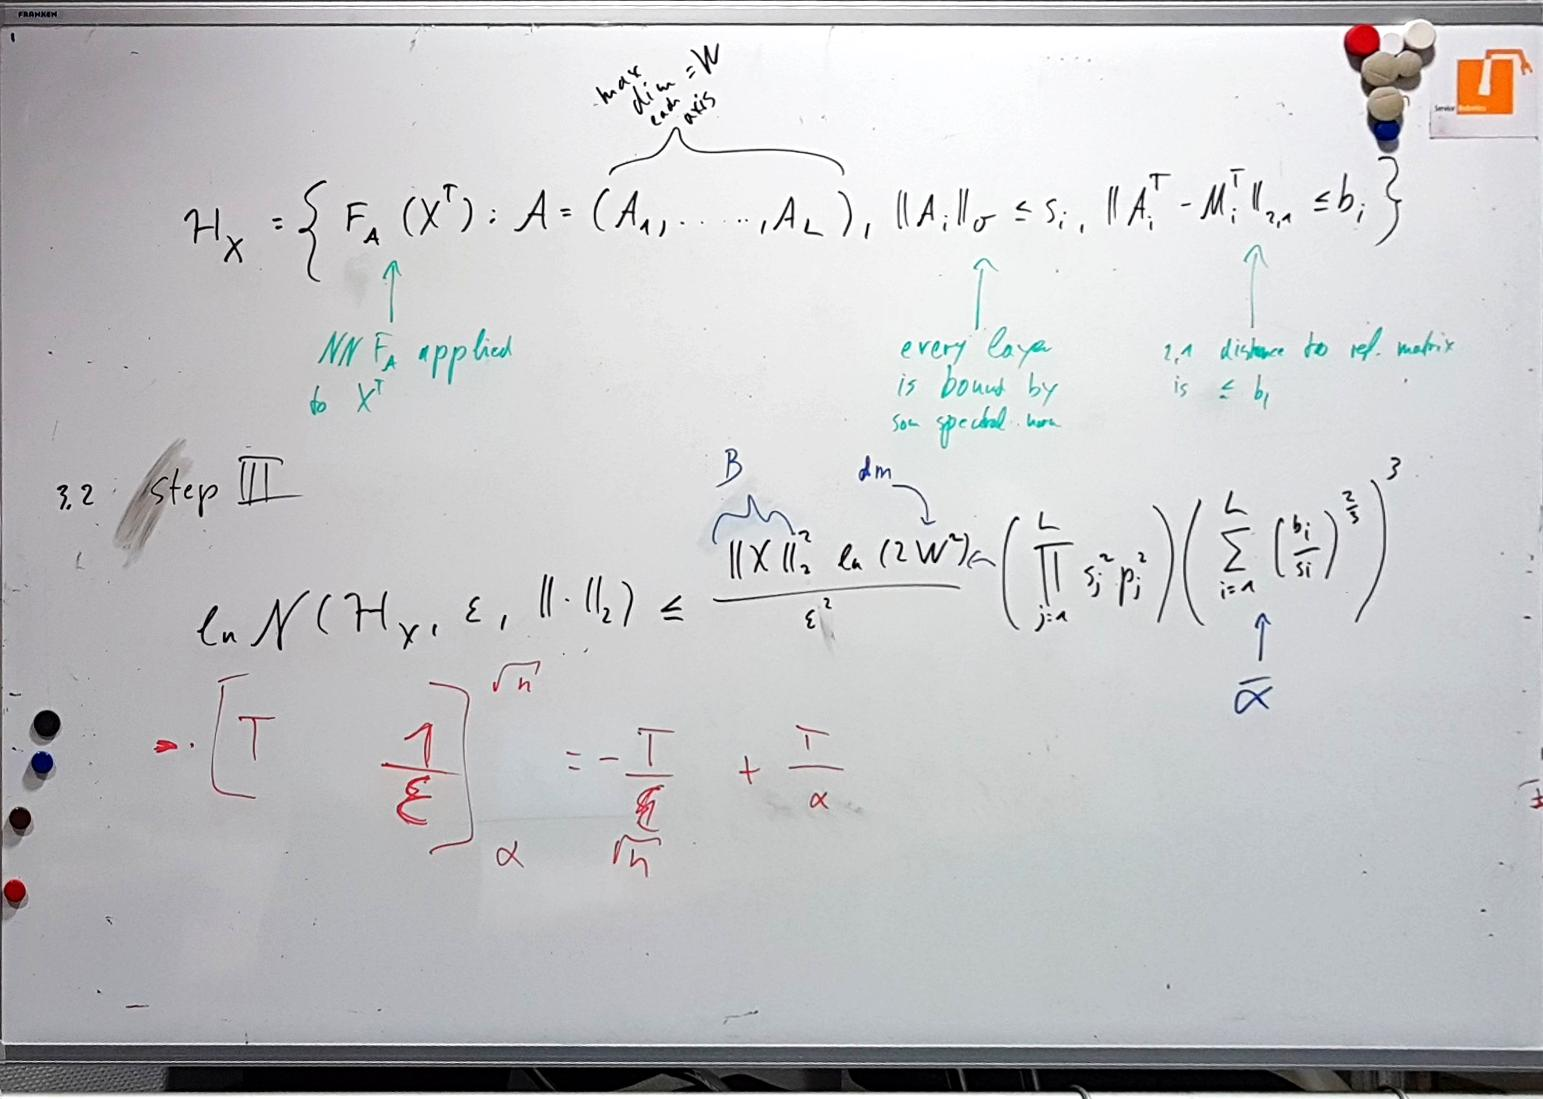
\includegraphics[width=\textwidth]{whiteboard_notes/20.jpg}
\end{figure}

\begin{figure}[htb]
	\centering
	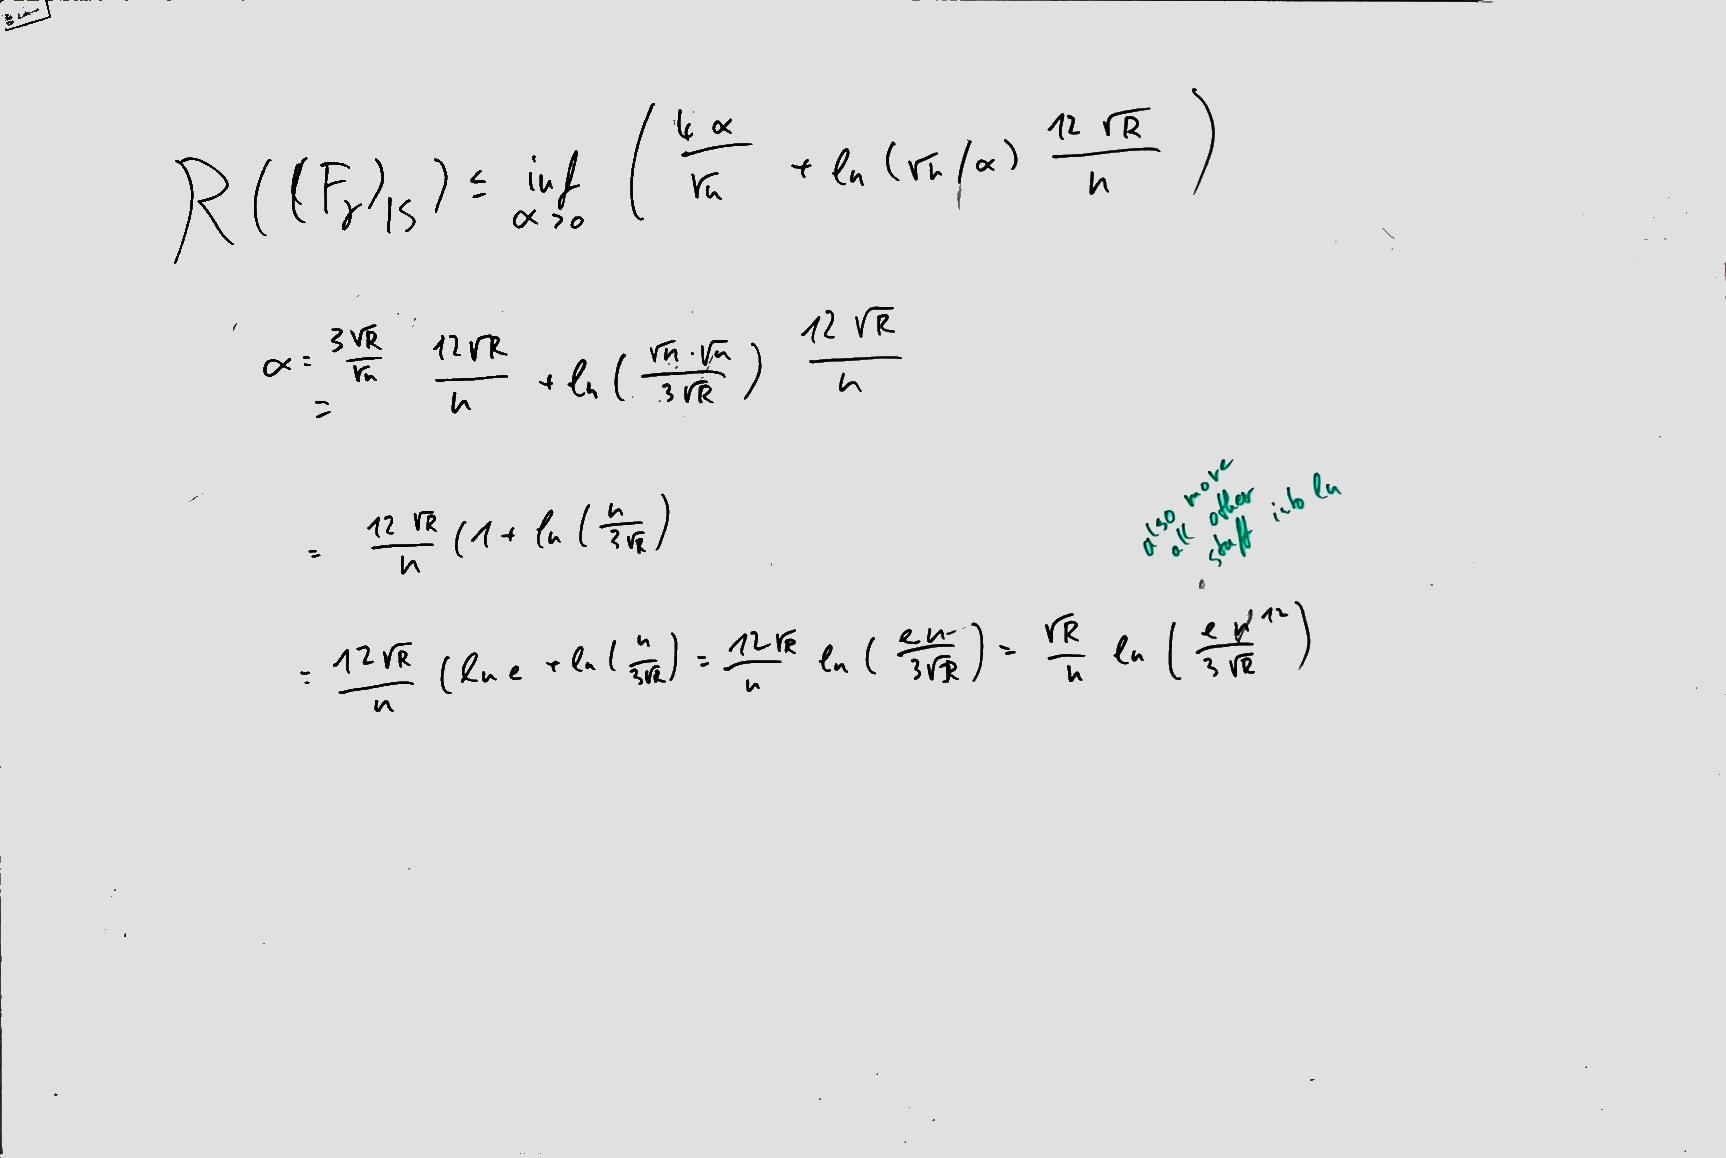
\includegraphics[width=\textwidth]{whiteboard_notes/21.jpg}
\end{figure}